% ============================================================================
% Korean Resume Template with Profile Photo
% Based on Sample.pdf - Saramin/JobKorea Standard Format
% Engine: XeLaTeX + kotex
% ============================================================================

\documentclass[a4paper, 10pt]{article}

% ============================================================================
% PACKAGES
% ============================================================================

\usepackage{kotex}
\usepackage{fontspec}
\usepackage[a4paper, top=15mm, bottom=15mm, left=20mm, right=20mm]{geometry}
\usepackage{tabularx}
\usepackage{array}
\usepackage{graphicx}
\usepackage{xcolor}
\usepackage[hidelinks]{hyperref}
\usepackage{calc}

% ============================================================================
% FONTS
% ============================================================================

\setmainfont{Malgun Gothic}[Script=Hangul, Language=Korean]
\setmainhangulfont{Malgun Gothic}
\setsanshangulfont{Malgun Gothic}

% ============================================================================
% PAGE SETUP
% ============================================================================

\pagestyle{empty}
\setlength{\parindent}{0pt}
\setlength{\parskip}{0pt}
\setlength{\baselineskip}{1.0\baselineskip}

% ============================================================================
% COLORS
% ============================================================================

\definecolor{darkgray}{RGB}{80, 80, 80}

% ============================================================================
% SECTION FORMATTING
% ============================================================================

\newcommand{\resumesection}[1]{%
  \vspace{8pt}
  \noindent
  {\large\bfseries #1}
  \vspace{2pt}
  \noindent\hrule
  \vspace{4pt}
}

% ============================================================================
% DOCUMENT START
% ============================================================================

\begin{document}

% ============================================================================
% HEADER WITH NAME AND PHOTO
% ============================================================================

\begin{minipage}[t]{0.70\textwidth}
  \vspace{0pt}
  {\fontsize{32}{32}\selectfont\textbf{조\ 동\ 휘}}

  \vspace{2pt}

  {\large JO DONGHWI}

  \vspace{4pt}
  \noindent\hrule
  \vspace{6pt}
\end{minipage}
\begin{minipage}[t]{0.28\textwidth}
  \vspace{0pt}
  \begin{center}
    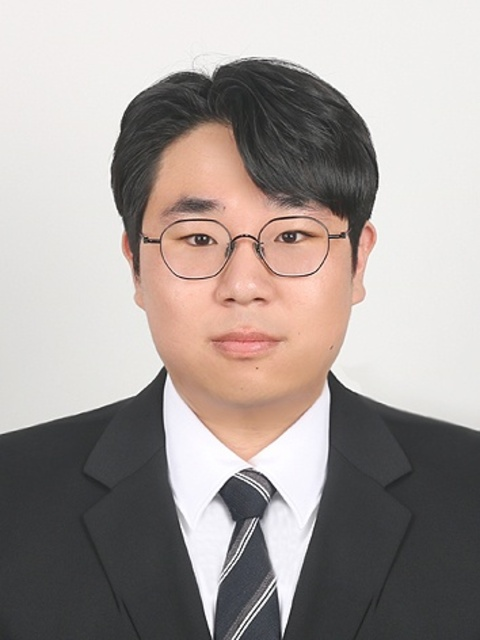
\includegraphics[width=3.2cm, height=4.2cm, keepaspectratio]{images/profile/증명사진.jpg}
  \end{center}
\end{minipage}

% ============================================================================
% PERSONAL INFORMATION
% ============================================================================

\resumesection{인\ 적\ 사\ 항}

\begin{tabularx}{\textwidth}{l X}
  생년월일 & 2000.08.10 (25세) \\
  현 주 소 & 서울특별시 관악구 신림로 30길 17-19 (올리하우스) 306호 \\
  연락처/이메일 & 010-8699-1510 / donghwi0711@icloud.com \\
  경력 & 1년 이상 (AI 소프트웨어 개발자) \\
\end{tabularx}

% ============================================================================
% EDUCATION
% ============================================================================

\resumesection{학\ 력\ 사\ 항}

\noindent
\begin{tabularx}{\textwidth}{l X l l}
  2021.03--2024.02 & 영남이공대학교 컴퓨터공학과 & 3.75/4.5 & 졸업 \\
  2016.03--2019.02 & 춘천기계공업고등학교 자동차과 & -- & 졸업 \\
\end{tabularx}

% ============================================================================
% WORK EXPERIENCE
% ============================================================================

\resumesection{경\ 력\ 사\ 항}

\vspace{2pt}
\noindent
\textbf{(주)토마토 \hfill 2024.04 -- 2025.01}

\noindent
\textbf{\quad 직위: 소프트웨어 엔지니어} \hfill 일본 도쿄도 시부야구

\begin{itemize}
  \setlength{\itemsep}{1pt}
  \setlength{\parskip}{0pt}
  \item AWS EC2 금융 시스템 인프라 구축 및 Windows Server/SQL Server 환경 설정
  \item Visual Studio 설치 SOP 작성으로 설치 시간 14\% 단축 달성
\end{itemize}

% ============================================================================
% EDUCATION & TRAINING
% ============================================================================

\resumesection{교\ 육\ 및\ 연\ 수}

\vspace{2pt}
\noindent
\textbf{SK Networks Family AI 캠프 \hfill 2026.01.20--2026.07.16}

\noindent
{\small PlayData / Encore / SK Networks | LLM 및 RAG 기술을 활용한 AI 부트캠프 (현재 진행 중)}

\vspace{3pt}
\noindent
\textbf{MLOps 과정 \hfill 2023.07.17--2023.08.11}

\noindent
{\small 동북권 ICT | ML 개발 로깅 및 배포 관리 시스템 학습}

\vspace{3pt}
\noindent
\textbf{실무프로젝트 드론+AI 과정 \hfill 2021.06.26--2021.08.14}

\noindent
{\small 대구 AI HUB | Jetson Nano 활용 OpenCV 실습 및 AI 도메인 융합 학습}

% ============================================================================
% AWARDS & ACTIVITIES
% ============================================================================

\resumesection{수\ 상\ 및\ 활\ 동}

\vspace{2pt}
\noindent
\textbf{\underline{수상}}

\vspace{2pt}
\noindent
\textbf{2021 \hfill 영남이공대학교 창업동아리 경진대회 - 스마트 헬멧} \hfill 최우수상 (14개팀 중 2등)

\vspace{1pt}
\noindent
\textbf{2022 \hfill 영남이공대학교 창업동아리 경진대회 - 키오스크 교육} \hfill 장려상 (중간평가)

\vspace{1pt}
\noindent
\textbf{2022 \hfill 맨드로바 메이커톤 2022 - 아이디어 상} \hfill 맨드로바

\vspace{4pt}
\noindent
\textbf{\underline{활동}}

\vspace{2pt}
\noindent
\textbf{N.A.P (Networks Application Programming)}

\noindent
{\small 전공 동아리 \& 창업 동아리 (2021.03 -- 2022.12) | 2021-2022 창업동아리 경진대회 참여}

\vspace{3pt}
\noindent
\textbf{스마트시티 프로젝트}

\noindent
{\small 제대로리빙랩 도시문제발굴단 (2022.08 -- 2022.09) | 대구시 장애인 콜택시 문제점 발견 및 해결방안 제시}

\vspace{3pt}
\noindent
\textbf{미래산업 수요특화 VR 교육}

\noindent
{\small 45시간 VR 부트캠프 수료 (2021.07) | 언리얼 엔진 4를 활용한 게임 및 콘텐츠 개발}

% ============================================================================
% MISCELLANEOUS (Other Information)
% ============================================================================

\resumesection{기\ 타\ 사\ 항}

\vspace{3pt}
\noindent
\textbf{언어 능력} \hfill JLPT (일본어능력시험) N3 (2023.01.12)

\vspace{2pt}
\noindent
\textbf{병역 사항} \hfill 2019.02 -- 2020.06 의병전역 (5급)

\vspace{2pt}
\noindent
\textbf{자격 사항}

\begin{itemize}
  \setlength{\itemsep}{1pt}
  \setlength{\parskip}{0pt}
  \item MOS (Microsoft Office Specialist) - Excel \hfill Microsoft (2021.06.04)
  \item 빅데이터전문가 1급 \hfill 한국직업능력검정협회 (2021.06.08)
\end{itemize}

\vspace{2pt}
\noindent
\textbf{취미 \& 특기} \hfill 애니메이션, 영화, 노래, 코딩


\end{document}
